\documentclass[xcolor=table]{beamer}
\usepackage[utf8]{inputenc}
\usepackage[british]{babel}
\usepackage[super]{nth}
%\usetheme{Boadilla}
%\usecolortheme{rose}
%\usecolortheme{crane}
\usefonttheme{structuresmallcapsserif}
\setbeamertemplate{navigation symbols}{}

\definecolor{Main}{rgb}{0.74, 0.13, 0.19}
\definecolor{Accent1}{rgb}{0.76,0.36,0.13}
\definecolor{Accent2}{rgb}{0.54,0.1,0.4}

\usecolortheme{rose}
%\useinnertheme[shadow]{circles}
\usecolortheme{whale}
%\useoutertheme{infolines}

\usecolortheme[named=Accent1]{structure}

\setbeamercolor{alerted text}{fg=Accent2}
%\setbeamercolor{palette primary}{fg=white}
%\setbeamercolor{palette secondary}{bg=Accent1}
%\setbeamercolor{palette tertiary}{bg=Accent2,fg=white}


\setbeamerfont{page number in head/foot}{size=\large}
\setbeamercolor{page number in head/foot}{fg=Main}
% page/total
%\setbeamertemplate{footline}[frame number]
% pas de total
\setbeamertemplate{footline}{%
    	\hfill%
	\usebeamercolor[fg]{page number in head/foot}%
	\usebeamerfont{page number in head/foot}%
	\insertframenumber\kern1em\vskip2pt%
}

\setbeamersize{text margin left=1em}
\setbeamersize{text margin right=1em}

%font
\usepackage[T1]{fontenc}
\usepackage[oldstylenums]{kpfonts}


%proper math and math symbols
%\usepackage{amsmath}
\usepackage{amssymb}

\usepackage{datenumber,fp}

\usepackage{siunitx}

\usepackage{tabu}
\usepackage{multirow}
\usepackage{booktabs}

% Allow the usage of graphics (.jpg, .png, etc.) in the document
\usepackage{graphicx}
\usepackage{tikz}
\usetikzlibrary{arrows,shapes,backgrounds, positioning, intersections, decorations.markings, decorations.shapes, mindmap, shapes.geometric, matrix, patterns}

\usepackage{pgfplots}
\usepackage{pgfplotstable}
\pgfplotsset{compat=1.9}
\usepgfplotslibrary{groupplots}
\usepgfplotslibrary{external}
\makeatletter
\newcommand*{\overlaynumber}{\number\beamer@slideinframe}
\tikzset{
  beamer externalizing/.style={%
    execute at end picture={%
      \tikzifexternalizing{%
        \ifbeamer@anotherslide
        \pgfexternalstorecommand{\string\global\string\beamer@anotherslidetrue}%
        \fi
      }{}%
    }%
  },
  external/optimize=false
}
\let\orig@tikzsetnextfilename=\tikzsetnextfilename
\renewcommand\tikzsetnextfilename[1]{\orig@tikzsetnextfilename{#1-\overlaynumber}}
\makeatother

\tikzset{every picture/.style={beamer externalizing}}
\tikzexternalize
\tikzsetexternalprefix{figs/}
%\tikzset{external/optimize=false}
%\tikzset{external/force remake}


%link or play movies
\usepackage{multimedia}



%beamer related package

\usepackage{todonotes}
\presetkeys{todonotes}{inline}{}


%bibliography
\usepackage[style=authoryear-comp, language=british,eprint=false, url=false, doi=false, sortcites=true, sorting=none, isbn=false, firstinits=true,maxcitenames=6]{biblatex}
%minimal citations
\AtEveryCitekey{%
	\clearfield{title}
	\clearfield{pages}
	\clearfield{volume}
	\clearfield{number}
	\clearfield{month}}
\newcommand{\myfullcite}[1]{{\scriptsize\fullcite{#1}}}
\renewbibmacro{in:}{%
  \ifentrytype{article}{}{%
  \printtext{\bibstring{in}\intitlepunct}}}
%\bibliography{biblio}

\institute{Liquides aux intefaces}
\title{Méthode de localisation et de mesure de particules colloïdales}
\author[M. Leocmach]{Mathieu Leocmach}
\date{12 Novembre 2015}
\titlegraphic{\footnotesize{\it Leocmach \& Tanaka, Soft Matter 2013}}

\begin{document}
\tikzset{every mark/.append style={scale=0.8}}
\pgfplotsset{every axis/.append style={small}}

\AtBeginSection[]{
	\addtocounter{framenumber}{-1}
	\begin{frame}[plain]
		\tableofcontents[currentsection, hideothersubsections]
	\end{frame}
}

\begin{frame}[plain]
	\titlepage
\end{frame}

\begin{frame}[plain]
	\tableofcontents[hidesubsections]
\end{frame}
\setcounter{framenumber}{0}

\section{Multiscale tracking}

\begin{frame}{Colloids as model atoms}
	\begin{columns}
	\column{0.5\textwidth}
	\begin{block}{Colloids are used as "experimental simulations" of statistical physics}
	\begin{itemize}
	\item Hard spheres
	\item Sticky spheres (short range attraction)
	\item Repulsive sphere (long range repulsion)
	\item Mixtures
	\item External fields
	\end{itemize}
	\end{block}
	
	\column{0.5\textwidth}
	Rich phase diagram mimicking atomic systems.
%	\begin{itemize}
%	\item Colloidal gas
%	\item Colloidal liquid
%	\item Colloidal crystal(s)
%	\item Colloidal glass
%	\item Colloidal gel
%	\end{itemize}
	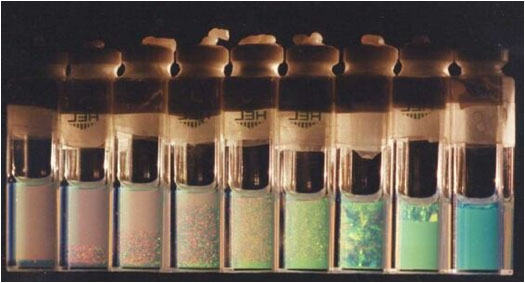
\includegraphics[width=\columnwidth]{Pusey_vanMegen}\\
	\footnotesize{\it Pusey \& van Megen, Nature (1986)}
	
	But also technologically useful in themselves.
	\end{columns}
\end{frame}

\begin{frame}{Confocal microscopy}
	\begin{center}\begin{columns}[c]
	\column{0.4\textwidth}
	\tikzsetnextfilename{confocal}
	\let\unitlength\relax
\newlength\unitlength
\setlength{\unitlength}{13\baselineskip}
	\begin{tikzpicture}[
		font=\footnotesize, 
		decoration={markings, mark=between positions 0.1 and 1 step 0.2\unitlength with {\arrow{stealth}}},
	]
	\draw[thick] (-0.12\unitlength,0) -- (-0.012\unitlength,0) (0.012\unitlength,0) -- (0.12\unitlength,0);
	\node[left] at (-0.12\unitlength,0) {aperture};
	\fill[name path=dichro, cyan, rotate around={-45:(0,-0.35\unitlength)}]  (-0.2\unitlength,-0.34\unitlength) rectangle (0.2\unitlength,-0.36\unitlength) (0, -0.34\unitlength) node[above, black, rotate=-45] {beam splitter};
	\draw[thick] (-0.35\unitlength,-0.23\unitlength) -- (-0.35\unitlength,-0.348\unitlength) (-0.35\unitlength,-0.362\unitlength) -- (-0.35\unitlength,-0.47\unitlength);
	\node[above] at (-0.35\unitlength,-0.23\unitlength) {pinhole};
	\fill[cyan] (0, -\unitlength) arc (-90:-70:0.6\unitlength) node (lensright) {} 
		arc (70:110:0.6\unitlength) node (lensleft) {}
		arc (-110:-90:0.6\unitlength);
	\path[name path=lensbottom] (lensleft) arc (-110:-70:0.6\unitlength);
	\path[name path=lenstop] (lensright) arc (70:110:0.6\unitlength);
	\fill[orange] (-0.15\unitlength, -1.05\unitlength) rectangle (0.15\unitlength, -1.15\unitlength);
	\draw[dashed] (-0.2\unitlength, -1.08\unitlength) -- (0.2\unitlength, -1.08\unitlength);
	\node[left] at (-0.2\unitlength, -1.08\unitlength) {focal plane};
	\node[above] at (0,0.1\unitlength) {light source};
	\path[name path=iray1] (0.012\unitlength, 0.1\unitlength) -- (-0.12\unitlength, -\unitlength);
	\path[name path=iray2] (0, -1.08\unitlength) -- (-0.15\unitlength, -0.95\unitlength);
	\path[name path=iray3] (-0.012\unitlength, 0.1\unitlength) -- (0.12\unitlength, -\unitlength);
	\path[name path=iray4] (0, -1.08\unitlength) -- (0.15\unitlength, -0.95\unitlength);
	\draw[
		postaction={decorate}, green!80!black,
		name intersections={of=iray1 and dichro, by=x},
		name intersections={of=iray3 and dichro, by=y},
		]
		(0.012\unitlength, 0.1\unitlength) -- (x)
		(-0.012\unitlength, 0.1\unitlength) -- (y);
		
	\draw[
		postaction={decorate}, green!80!black, dashed, dash pattern=on 5pt off 5pt, dash phase=0pt,
		name intersections={of=iray1 and dichro, by=x}, 
		name intersections={of=iray1 and lenstop, by=a}, 
		name intersections={of=iray2 and lensbottom, by=b},
		name intersections={of=iray4 and lensbottom, by=c},
		name intersections={of=iray3 and lenstop, by=d},
		name intersections={of=iray3 and dichro, by=y},
		] 
		(x) -- (a) -- (b) -- (0, -1.08\unitlength)
		(y) -- (d) -- (c) -- (0, -1.08\unitlength);
	\draw[postaction={decorate}, red!80!black, 
		name intersections={of=iray1 and dichro, by=x}, 
		name intersections={of=iray3 and dichro, by=y},
		] 
		(x) -- (-0.41\unitlength, -0.362\unitlength) 
		(y) -- (-0.41\unitlength, -0.348\unitlength);
	\draw[postaction={decorate}, red!80!black, dashed, dash pattern=on 5pt off 5pt, dash phase=10pt,
		name intersections={of=iray1 and dichro, by=x}, 
		name intersections={of=iray1 and lenstop, by=a}, 
		name intersections={of=iray2 and lensbottom, by=b},
		name intersections={of=iray4 and lensbottom, by=c},
		name intersections={of=iray3 and lenstop, by=d},
		name intersections={of=iray3 and dichro, by=y},
		] 
		(0, -1.08\unitlength) -- (b) -- (a) -- (x) 
		(0, -1.08\unitlength) -- (c) -- (d) -- (y);
	\draw[thick, blue] (-0.39\unitlength, -0.33\unitlength) arc (90:270:0.025\unitlength);
	\node[above left, rotate=90] at (-0.39\unitlength, -0.33\unitlength) {light detector};
	\path[name path=badray1] (0,0) -- (-0.18\unitlength, -1.1\unitlength);
	\path[name path=badray2] (0, -1.12\unitlength) -- (-0.3\unitlength, -0.85\unitlength);
	\path[name path=badray3] (0,0) -- (0.18\unitlength, -1.1\unitlength);	
	\path[name path=badray4] (0, -1.12\unitlength) -- (0.3\unitlength, -0.85\unitlength);
	\draw[dotted,
		name intersections={of=badray1 and dichro, by=x}, 
		name intersections={of=badray1 and lenstop, by=a}, 
		name intersections={of=badray2 and lensbottom, by=b},
		name intersections={of=badray4 and lensbottom, by=c},
		name intersections={of=badray3 and lenstop, by=d},
		name intersections={of=badray3 and dichro, by=y},
		] 
		(0, -1.12\unitlength) -- (b) -- (a) -- (x) --  (-0.35\unitlength, -0.38\unitlength)
		(0, -1.12\unitlength) -- (c) -- (d) -- (y) --  (-0.35\unitlength, -0.33\unitlength);
	\end{tikzpicture}
	\column{0.5\textwidth}
	\begin{tabular}{lm{0.5\columnwidth}}
		$XY$ slice & 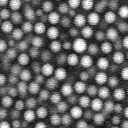
\includegraphics[width=0.5\columnwidth]{sliceXY} \\
		$XZ$ slice & 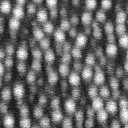
\includegraphics[width=0.5\columnwidth]{sliceXZ} \\
	\end{tabular}
	\end{columns}\end{center}
\end{frame}

\begin{frame}{Monodisperse particle tracking}
	\begin{columns}[T]
	\column{0.3\textwidth}
	Original image\\
	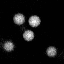
\includegraphics[width=\textwidth]{dillute_raw}
	
	\bigskip
	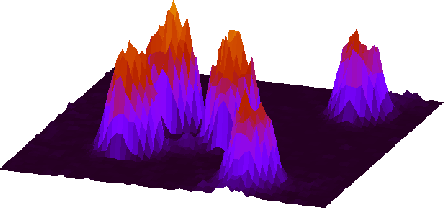
\includegraphics[width=\textwidth]{dillute_raw_gp_raster}
	\column{0.3\textwidth}
	Blurred\\
	
\includegraphics[width=\textwidth]{dillute_filtered}
	
	\bigskip
	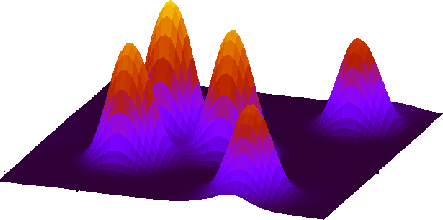
\includegraphics[width=\textwidth]{dillute_filtered_gp_raster}
	\column{0.3\textwidth}
	Local maxima\\
	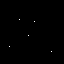
\includegraphics[width=\textwidth]{dillute_centers}
	
	\bigskip
	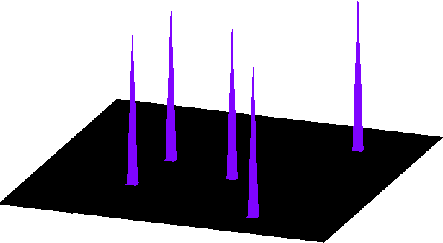
\includegraphics[width=\textwidth]{dillute_centers_gp_raster}
	\end{columns}
	
	
	Resolution up to $\SI{1/10}{px}$ via subpixel resolution methods.
	
	\bigskip
	
	\footnotesize{\it Crocker \& Grier J. Coll. Interf. Sci. (1996)}
\end{frame}

\begin{frame}{Monodisperse particle tracking}
	\begin{columns}[T]
	\column{0.3\textwidth}
	\centering
	Not enough blur\\
	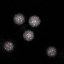
\includegraphics[width=\textwidth]{dillute_notblured}
	\column{0.3\textwidth}
	\centering
	Good blur\\
	\tikzsetnextfilename{good_blur_mono}
		\begin{tikzpicture}
		\node[inner sep=0, anchor=south west]{
\includegraphics[width=\textwidth]{dillute_filtered}};
		\fill[red!50!white] (9/64.0*\textwidth, 17/64.0*\textwidth) rectangle (10/64.0*\textwidth, 18/64.0*\textwidth);
		\fill[red!50!white] (19/64.0*\textwidth, 44/64.0*\textwidth) rectangle (20/64.0*\textwidth, 45/64.0*\textwidth);
		\fill[red!50!white] (28/64.0*\textwidth, 27/64.0*\textwidth) rectangle (29/64.0*\textwidth, 28/64.0*\textwidth);
		\fill[red!50!white] (34/64.0*\textwidth, 42/64.0*\textwidth) rectangle (35/64.0*\textwidth, 43/64.0*\textwidth);
		\fill[red!50!white] (51/64.0*\textwidth, 11/64.0*\textwidth) rectangle (52/64.0*\textwidth, 12/64.0*\textwidth);
	\end{tikzpicture}
	\column{0.3\textwidth}
	\centering
	Too much blur\\
	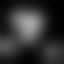
\includegraphics[width=\textwidth]{dillute_tooblured}
	\end{columns}
	\begin{itemize}
	\item We must choose \alert{the right} blurring radius.
	\item Ok for monodisperse particles
	\item Problematic for polydisperse
	\end{itemize}
\end{frame}

\begin{frame}{Same method with polydisperse particles}
	\begin{columns}[T]
	\column{0.3\textwidth}
	\centering
	{\strut{}Multiple centres}\\
	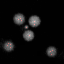
\includegraphics[width=\textwidth]{dillute_smaller_blur0_5}
	\column{0.3\textwidth}
	\centering
	{\strut{}Misplaced centres}\\
	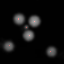
\includegraphics[width=\textwidth]{dillute_smaller_blur1}
	\column{0.3\textwidth}
	\centering
	{\strut{}Overlook small}\\
	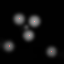
\includegraphics[width=\textwidth]{dillute_smaller_blur1_5}
	\end{columns}
	\begin{itemize}
	\item There is no \alert{right} blurring radius $\Rightarrow$ We always have errors.
	\item We cannot extract the sizes of the particles, important for the physics of the system.
	\begin{itemize}
		\item Volume fraction
		\item Neighbours
	\end{itemize}
	\end{itemize}
\end{frame}

\begin{frame}{Not better in 3D}
	\begin{center}
	\begin{tabular}{ccc}
	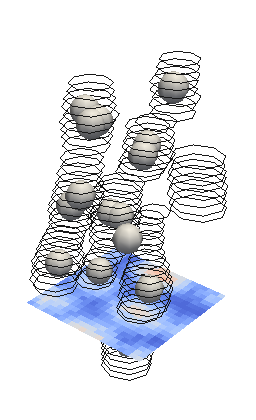
\includegraphics[width=0.18\textwidth]{comp3D_monoscale_r20_crop} & %
	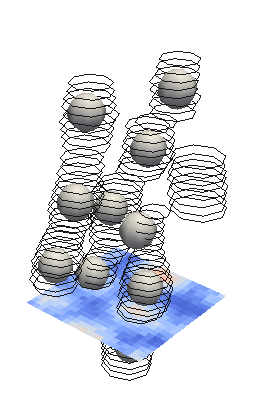
\includegraphics[width=0.18\textwidth]{comp3D_monoscale_r25_crop} & %
	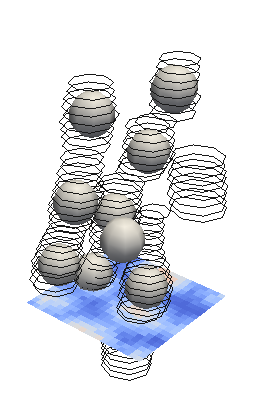
\includegraphics[width=0.18\textwidth]{comp3D_monoscale_r30_crop} \\ 
	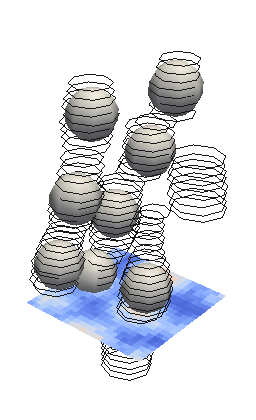
\includegraphics[width=0.18\textwidth]{comp3D_monoscale_r35_crop} & %
	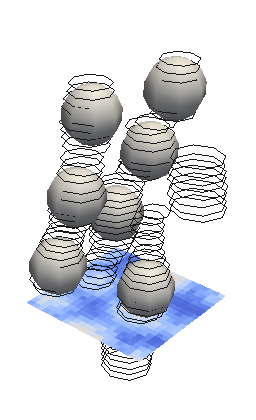
\includegraphics[width=0.18\textwidth]{comp3D_monoscale_r40_crop} & %
	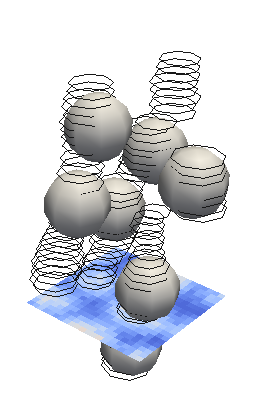
\includegraphics[width=0.18\textwidth]{comp3D_monoscale_r45_crop} \\ 
	\end{tabular} 
	\end{center}
\end{frame}

\begin{frame}{Scale space}
	\footnotesize{Scale space, \footnotesize{\it Lindeberg, Int. J. Comput. Vis. (1993)}\\ Scale-invariant feature transform, \footnotesize{\it Lowe, Int. J. Comput. Vis. (2004)}}
	
	\tikzsetnextfilename{scale_space_1D}
		\begin{tikzpicture}[%
		minus/.style={
			shape=circle, draw, inner sep=0, %
			text height=1.5ex,text depth=.25ex,%
			node distance=0.5%
			},%
		]
		\begin{groupplot}[%
			group style={
				group size=2 by 1,%
				},%
			anchor=north,%
			width=0.5\textwidth,%
			xtick=\empty, ytick=\empty,%
			xlabel={position}, xlabel near ticks, ylabel near ticks, %
			no markers,
			title style={text height=1.5ex,text depth=.25ex, anchor=center},%
			]
			\nextgroupplot[%
				ylabel={intensity},%
				title={Increasing Gaussian blur},%
			]
				\addplot[black] table[x expr=\coordindex, y expr=\thisrowno{0}]{gaussians.txt};
				\addplot[blue] table[x expr=\coordindex, y expr=\thisrowno{1}-2]{gaussians.txt};
				\node at (current plot end) (g1) {};
				\addplot[blue!67!red] table[x expr=\coordindex, y expr=\thisrowno{2}-4]{gaussians.txt};
				\node at (current plot end) (g2) {};
				\addplot[blue!33!red] table[x expr=\coordindex, y expr=\thisrowno{3}-6]{gaussians.txt};
				\node at (current plot end) (g3) {};
				\addplot[red] table[x expr=\coordindex, y expr=\thisrowno{4}-8]{gaussians.txt};
				\node at (current plot end) (g4) {};
				
			\only<1>{
			\nextgroupplot[%
				title={Difference of Gaussians},%
				ymax=0.45,%
			]
				\addplot+[smooth, blue] table[x expr=\coordindex, y expr=\thisrowno{2}-\thisrowno{1}]{gaussians.txt};
				\node at (current plot begin) (DoG1) {};
				\addplot+[smooth, blue!67!red] table[x expr=\coordindex, y expr=\thisrowno{3}-\thisrowno{2}-0.2]{gaussians.txt};
				\node at (current plot begin) (DoG2) {};
				\addplot+[smooth, blue!33!red] table[x expr=\coordindex, y expr=\thisrowno{4}-\thisrowno{3}-0.4]{gaussians.txt};
				\node at (current plot begin) (DoG3) {};
			}
			\only<2>{
			\nextgroupplot[%
				title={Difference of Gaussians},%
			]
				\addplot+[smooth, blue] table[x expr=\coordindex, y expr=\thisrowno{2}-\thisrowno{1}]{gaussians.txt};
				\addplot+[smooth, blue!67!red] table[x expr=\coordindex, y expr=\thisrowno{3}-\thisrowno{2}]{gaussians.txt};
				\node at (current plot begin) (DoG2) {};
				\addplot+[smooth, blue!33!red] table[x expr=\coordindex, y expr=\thisrowno{4}-\thisrowno{3}]{gaussians.txt};
				\draw[->, thick] (rel axis cs:0.5,0.0015) -- (rel axis cs:0.5,0.075);
			}
				
		\end{groupplot}
		\only<1>{
		\node[minus, blue] (diff1) [left=of DoG1] {-};
		\draw [->, blue] (g1) -- (diff1);
		\draw [->, blue!67!red] (g2) -- (diff1);
		\draw [->, blue] (diff1) -- (DoG1);
		}
		\node[minus, blue!67!red] (diff2) [left=of DoG2] {-};
		\draw [->, blue!67!red] (g2) -- (diff2);
		\draw [->, blue!33!red] (g3) -- (diff2);
		\draw [->, blue!67!red] (diff2) -- (DoG2);
		\only<1>{
		\node[minus, blue!33!red] (diff3) [left=of DoG3] {-};
		\draw [->, blue!33!red] (g3) -- (diff3);
		\draw [->, red] (g4) -- (diff3);
		\draw [->, blue!33!red] (diff3) -- (DoG3);
		}
	\end{tikzpicture}
	
	\begin{itemize}
		\item The magnitude of the DoG should be maximized at the center of the blob.
		\item<2> The optimal scale, which depends on the size of the blob, should be detected.
	\end{itemize}
\end{frame}

\begin{frame}{Locating particles in both scale and space}
	\begin{columns}[T]
	\column{0.7\textwidth}
	\def\svgwidth{\columnwidth}
	\input{sift_octave1.pdf_tex}
	\def\svgwidth{\columnwidth}
	\input{sift_octave0.pdf_tex}
	\column{0.3\textwidth}
	\def\svgwidth{\columnwidth}
	\input{sift_localmin.pdf_tex}
	Minima of the DoG images are detected by neighbourhood search.
	\end{columns}
	
	%\footnotesize{\citet{Lindeberg1993, Lowe2004}}
\end{frame}



\begin{frame}{Optimal scale}
	For a binary disk of radius $R$, the DoG response is minimum for a scale $\sigma^{*} \propto R$. The proportionality constant is known analytically.
	
	\tikzsetnextfilename{binary_disk}
	\begin{tikzpicture}
		\begin{axis}[
			name=a,
			width=0.55\columnwidth,%
			xmin=0, ymax=0, xmax=5, %
			xlabel=$R/\sigma^*$, ytick={0},%
			ylabel={DoG response}, ylabel near ticks, %
			no marks,%
			]
			\addplot+[smooth] {exp(-x^2/2) - exp(-x^2/2/2^(2/3))};
		\end{axis}

\node[fill=black, anchor=north west, minimum width=0.4\columnwidth, minimum height=0.4\columnwidth] (r) at ($(a.right of north east) + (-\columnwidth,0)$) {};
\node[fill=white, circle, minimum width=0.2\columnwidth] at (r) (c) {};
\draw[->, Accent1, thick] (c.center) -- (c.east) node[midway, below] {$R$};

\end{tikzpicture}
\end{frame}

\begin{frame}{Isolated sphere}
	\tikzsetnextfilename{io_radius}
	\begin{tikzpicture}
	\pgfplotsset{cycle list name=black white, clip marker paths=true,}
	\begin{groupplot}[%
		group style={
				group name=g, group size=2 by 1,
				horizontal sep=5em,
				},
		width=0.5\columnwidth,%
		height=0.5\columnwidth,%
		xlabel={Input radius (px)}, 
		extra x ticks={3.47}, extra x tick labels={}, extra tick style={grid=major},%
		]
		\nextgroupplot[ylabel={Output radius}, ytick={2,4,...,14},]
		\addplot+[only marks, mark size=0.5, mark=o] table [x index=0, y expr ={\thisrowno{1}}] {multiscale_relative_sizes.out};
		\addplot+[no marks, domain=1.5:14] {x};
	
	\nextgroupplot[%
        ylabel={$R$ relative error (\%)},%
		extra y ticks={0}, extra y tick labels={},%
		]
		\addplot table [x index=0, y expr ={100*(\thisrowno{1}/\thisrowno{0}-1)}] {multiscale_relative_sizes.out};
	\end{groupplot}
	\end{tikzpicture}
\end{frame}

\begin{frame}{Two spheres}
	%\tikzset{external/force remake=false}
	\begin{columns}[c]
	\column{0.55\textwidth}
	\tikzsetnextfilename{two_spheres}
		\begin{tikzpicture}
	\begin{groupplot}[%
		group style={
				group size=1 by 2,%
				x descriptions at=edge bottom,
				vertical sep=0.5em,
				},%
		height=0.5\textheight,%
		width=\columnwidth,%
		xlabel={$r_{ij}$ (px)}, 
		xmin=8, xmax=18, xtick={8,...,17},%
		extra tick style={grid=major},%
		]
		\nextgroupplot[%
			ylabel={$r_{ij}$ error (\SI{0.01}{px})},%
			extra y ticks={0}, extra y tick labels={},%
			]
		\addplot table [x index=0, y expr ={(\thisrowno{2}-\thisrowno{1}-\thisrowno{0})*100}] {close_neighbours3D.out};
		\draw (axis cs:12,-6) circle[radius=0.05\textwidth] (axis cs:16,-6) circle[radius=0.05\textwidth];
		\draw[dashed] (axis cs:12,-6) -- (axis cs:12,-9) (axis cs:16,-9) -- (axis cs:16,-6);
		\draw[<->] (axis cs:12,-9) -- (axis cs:16,-9) node[midway, above] {$r_{ij}$};
		\draw[->] (axis cs:11.05,-6) -- +(0,0.05\textwidth,0) node[midway, left] {\SI{4}{px}};
		\draw[->, very thick] (axis cs:16,-6) -- (axis cs:14,-6);
	
	\nextgroupplot[
		ylabel={$R$ (px)},%
		extra y ticks={4}, extra y tick labels={},%
		legend style={legend pos=south east}
		]
		\addplot table [x index=0, y index=4] {close_neighbours3D.out};
		\addplot+[mark=square] table [x index=0,y index=6] {close_neighbours3D.out};
		\legend{No correction, One iteration};
	\end{groupplot}
	\end{tikzpicture}
	\column{0.45\textwidth}
	Error at contact $\approx \SI{0.1}{px}$, like monodisperse tracking.
	
	\bigskip
	
	The DoG response at the center of particle $i$ is a superposition of the contribution of each (neighbouring) particle.
	\[
	%\forall i,\quad 
	DoG_i = \sum_j DoG(r_{ij}, R_j)
	\label{eq:superpos}
	\]
	\structure{Sparse system} solved iteratively
	\end{columns}
\end{frame}

\begin{frame}{Many particles}
	Simulation data of 5000 HS to generate image
	
	\tikzsetnextfilename{size_correction}
	\begin{tikzpicture}
	\pgfplotsset{cycle list name=black white, clip marker paths=true,}
	\begin{axis}[%
		name=finite,
		at={(0,-1.35\columnwidth)},%
		height=0.5\columnwidth,%
		width=\columnwidth,%
		area legend,
		const plot, no marks,%
		xlabel={$R$ (px)}, ylabel={Size distribution},%
		xtick={4.3, 4.4, ..., 5.4},
		extra tick style={grid=major},%
		extra x ticks={5.298}, extra x tick labels={},%
		ymin=0,%		
		legend style={legend pos=north west, cells={anchor=west}}
		]
		\addplot+[pattern=north west lines] file {john_exact_mono_large_init.hist} \closedcycle;
		\addplot+[red, fill=red, semitransparent] file {john_exact_mono_large_cor1.hist} \closedcycle;
		\addplot+[pattern=dots, pattern color=blue] file {john_exact_mono_large_cor2.hist};
		\legend{No correction, One iteration, Two iterations};
		\draw[decorate,decoration=brace] (axis cs:4.75, 200) -- (axis cs:5.05, 200) node[midway, above] {edges};
	\end{axis}
	\end{tikzpicture}
\end{frame}



\begin{frame}{Deconvolution}
	\begin{columns}[c]
	\column{0.66\textwidth}
	$y = x \star h + \epsilon$ with $h$ the point spread function.
	\tikzsetnextfilename{deconv_images}
	\begin{tikzpicture}
		\begin{groupplot}[%
		group style={
				group name=pics,
				group size=3 by 1,%
				horizontal sep=0.0075\textwidth,
				vertical sep=0.0075\textwidth,
				},%
		width=0.3\textwidth,%
		height=0.33\textwidth,%
		xmin=0,xmax=50,ymin=0,ymax=55,%
		axis lines=none,%
		scale only axis=true,%
		point meta=explicit symbolic,%
		scatter/@pre marker code/.code={%
        	\pgfmathparse{10*\pgfplotspointmetatransformed*\pgfplotsunitxlength}%
        	%\pgfplotstransformcoordinatex{\pgfplotspointmetatransformed}
            \def\markopts{mark=o,black,mark size=\pgfmathresult}%
            \expandafter\scope\expandafter[\markopts]
            },%
        scatter/@post marker code/.code={\endscope} 
		]
		\nextgroupplot[title={Original}]
			\addplot graphics [xmin=0,xmax=50,ymin=0,ymax=55]{Zelong_original};
		\nextgroupplot[title={Blurred}]
			\addplot graphics [xmin=0,xmax=50,ymin=0,ymax=55]{Zelong_blurred};
			\addplot+[only marks, scatter] table [x index=1, y expr={55-\thisrowno{2}}, meta index=3] {Z_elong.xyz};
		\nextgroupplot[title={Deconvolved}]
			\addplot graphics [xmin=0,xmax=50,ymin=0,ymax=55]{Zelong_deconvolved};
			\addplot+[only marks, scatter] table [x index=1, y expr={55-\thisrowno{2}}, meta index=3] {Z_elong_deconv.xyz};
		\end{groupplot}
	\end{tikzpicture}
	\begin{itemize}
	\item If the system is isotropic, the spectrum along $z$ must be the same as the spectrum along $x$ ou $y$.\\ $\Rightarrow$ Possible to measure the \textsc{psf}.
	\item No need to deconvolve the noisy original image, we can use the first Gaussian blurred version.
	\end{itemize}
	
	
	\column{0.33\textwidth}
	\tikzsetnextfilename{deconv_rdf}
	\begin{tikzpicture}
		\begin{axis}[%
			anchor=outer south west,
			width=\columnwidth,%
			height=0.9\textheight,%
			xlabel = {$r$ [\si{\micro\metre}]}, ylabel={$g(r)$},%
			xlabel near ticks, ylabel near ticks,
			xmin=0,xmax=4,ymin=0,%
			no marks,%
			]
			\addplot file {cp0.34.rdf};
			\addplot file {cp0.34_deconv.rdf};
		\end{axis}
	\end{tikzpicture}
	\end{columns}
\end{frame}

\section{Heterogeneous crystallisation}

\begin{frame}{Our colloids}
	\begin{columns}
	\column{0.5\textwidth}
	\begin{center}
	\rotatebox{90}{\qquad \small{SEM image}}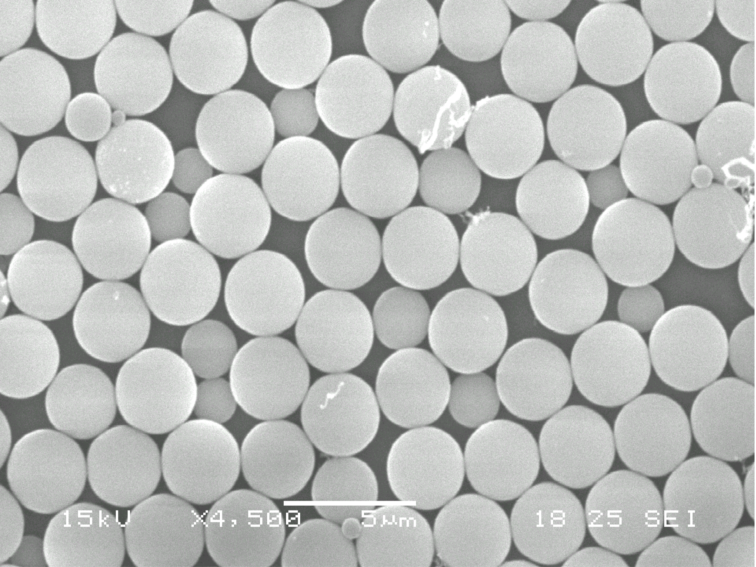
\includegraphics[width=0.8\columnwidth, height=0.6\columnwidth]{SEM}
	\end{center}
	\structure{Solvent}
	\begin{itemize}
		\item Cis-decalin
		\item Cyclohexylbromide
	\end{itemize}
	Matching
	\begin{itemize}
		\item Optical index
		\item Density (with $T$ control)
	\end{itemize}
	\column{0.5\textwidth}
	\begin{block}{PMMA particles}
		\begin{itemize}
			\item $\sigma \simeq \SI{3.3}{\micro\metre}$
			\item $\Delta \simeq 6\%$ not Gaussian
		\end{itemize}
		Hard spheres
		\begin{itemize}
			\item Sterically stabilized
			\item Salt to screen charges\\ (Debye length $<\SI{100}{\nano\metre}$)
		\end{itemize}
	\end{block}
	\end{columns}
\end{frame}

\begin{frame}<1-3>{Size distribution}
	\tikzsetnextfilename{size_distrib}
	\begin{tikzpicture}
	\begin{axis}[%
		name=hist,
		width=\columnwidth, height=0.5\textheight,%
		%scale only axis,
		xlabel={Diameters [$\si{\micro\metre}$]},%
		xmin=1, xmax=5,
		axis y line*=left,
		ymin=0, ytick=\empty,%
		ylabel={Size distribution},%
		ylabel near ticks,
		legend style={legend pos=north west}, area legend,
		]
		\addplot[ybar, ybar interval, gray!50, fill=gray!50] file {SEM_size_distrib.txt} \closedcycle;
		\legend{\textsc{sem}}
	\end{axis}
	\only<2->{\begin{axis}[%
		name=hist2,
		width=\columnwidth, height=0.5\textheight,%
		xmin=1, xmax=5,
		axis y line*=right,
		ymin=0, ytick=\empty,%
		no marks,%
		]
		\addplot+[dashed] table[x expr ={2*\thisrow{r}}, y=all] {all_ico_icongb_mrco_X.rdist};
		\addlegendentry{In situ};
		\only<3>{\addplot table [x expr ={2*\thisrow{r}/1.25}, y index=1] {all_ico_icongb_mrco_X.rdist};}%
		\draw<3>[->, ultra thick] (axis cs:3.15,3) -- (axis cs: 3.9, 3) node[midway, above] {swelling};%
	\end{axis}}
	\end{tikzpicture}
\end{frame}

\begin{frame}{Are the sizes correct ?}
	\tikzsetnextfilename{size_check}
	\begin{tikzpicture}
	\begin{groupplot}[%
		group style={group size=2 by 1, horizontal sep=5em},%
		width=0.45\textwidth,%
		]
	\nextgroupplot[%
		xmin=2, xmax=6, xlabel={Optical radius [px]},%
		ymin=0, ymax=20,%
		ylabel={Position of the first peak of $g_R(r)$ [px]},
		y label style={align=center, text width=0.5\textheight},%
		]
		\addplot+[black,forget plot, no marks, domain=2:6] {3*x};
		\addplot+[black,only marks, mark=o] file {rdf_peak_pos_radius.out};
		
	\nextgroupplot[%
		%width=0.5\columnwidth, height=0.5\columnwidth,%
		xmin=0, xmax=1.5,%
		xlabel ={$r/\sigma_\text{peak}$, $\hat{r}$},%
		ymin=0,%
		ylabel=$g(r)$, ylabel near ticks,%
		no marks,%
		legend style={legend pos=north west}, 
		]
		\addplot+[dashed] file {yon6.rdf};
		\addplot file {yon6.srdf};
		\legend{$g(r)$, $g(\hat{r})$};
	\end{groupplot}
	\end{tikzpicture}

	
	Sizes $\Rightarrow\phi=0.60\Rightarrow$ Glass
\end{frame}

\begin{frame}{Structures in the glass}
	\tikzsetnextfilename{glass_structure}
	\begin{tikzpicture}
	\definecolor{BlueViolet}{rgb}{0.62352, 0.372549, 0.623529};
		\node[anchor=south east] (t000) {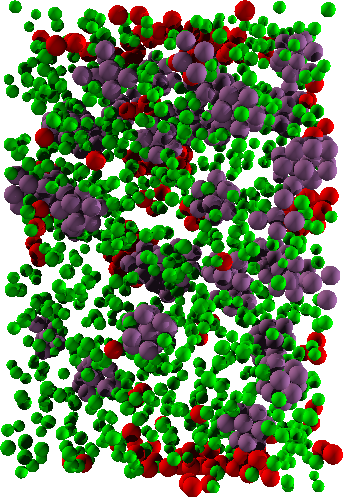
\includegraphics[height=0.7\textheight]{mrco_ico_small_t000.png}};
		\node[anchor=south west] (t299) {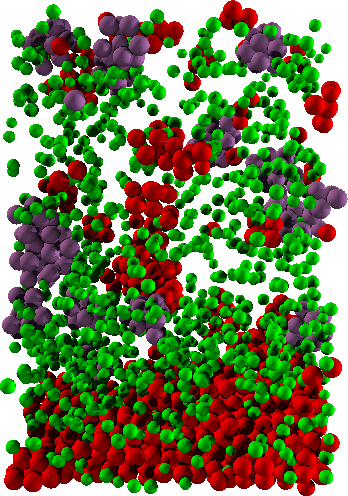
\includegraphics[height=0.7\textheight]{mrco_ico_small_t299.png}};
		\node[below=0 of t000.south] {$t=0$};
		\node[below=0 of t299.south] {$t=\SI{40}{\hour}$};
		\draw[->] (0,0.1\textheight) -- (0,0.5\textheight) node[above]{$z$};
		\matrix[%
		matrix of nodes, right=-0.5em of t299.east, ampersand replacement=\&,
		column 1/.style={right, text height=0.8em, text depth=0.2em},%
		column 2/.style={left, circle, shade, inner sep=0.008\textwidth},%
		] (l)
	{
		Crystal-like \& |[ball color=red]|{}\\
		Icosahedra \& |[ball color=BlueViolet]|{}\\
		Small \& |[ball color=green]|{}\\
	};
	\end{tikzpicture}
\end{frame}

\begin{frame}{Size distribution of the structures}
	\tikzsetnextfilename{size_distrib_struct}
	\begin{tikzpicture}
	\begin{groupplot}[%
		group style={
			group name=distrib,
			group size=1 by 2,
			},%
		width=\columnwidth,%
		height=0.5\textheight,%
		no marks,%
		xlabel={$R$ [\si{\micro\metre}]}, xmin=0.8, xmax=2.5,%
		ylabel={Size distribution}, ymin=0, ymax=12,%
		legend style={legend pos=north west},
		]
		\nextgroupplot
		\addplot table[x=r, y=all] {all_ico_icongb_mrco_X.rdist};
		\addplot table[x=r, y=mrco] {all_ico_icongb_mrco_X.rdist};
		\addplot table[x=r, y=X] {all_ico_icongb_mrco_X.rdist};
		\legend{all, \textsc{mrco}, crystalline};
		
		\nextgroupplot
		\addplot table[x=r, y=all] {all_ico_icongb_mrco_X.rdist};
		\addplot table[x=r, y=ico] {all_ico_icongb_mrco_X.rdist};
		\addplot table[x=r, y=icongb] {all_ico_icongb_mrco_X.rdist};
		\legend{all, ico. centre, ico. surf.};
	\end{groupplot}
	\end{tikzpicture}
	
\end{frame}


\begin{frame}[plain]
\end{frame}



\appendix
\newcounter{finalframe}
\setcounter{finalframe}{\value{framenumber}}

\begin{frame}{Density profiles}
	\tikzsetnextfilename{profiles}
	\begin{tikzpicture}
		\begin{groupplot}[%
			group style={
				group name=profiles,
				group size=2 by 2,
				y descriptions at=edge left,%
				x descriptions at=edge bottom,%
				horizontal sep=0,
				vertical sep=0,
			},%
			width=0.4\textwidth,
			height=0.45\textheight,%
			ymin=0, ymax=1,%
			ytick={0,0.2,...,1},%
			no marks,%
			ylabel near ticks,%
			xlabel=$z/(2R_\text{peak})$,%
			xmin=1, xmax=26,%
			axis on top,
			]
		\nextgroupplot[ylabel={$\rho$ large}]
		\addplot+[gray!50, fill=gray!50] table[x index=0, y index=1]{large_small_mrco_t000.gauss.zhist} \closedcycle;
		\addplot+[thick] table[x index=0, y index=3]{large_small_mrco_t000.gauss.zhist};
		\addplot+[black] table[x index=0, y index=1]{large_small_mrco_t000.zhist};
		\node at (rel axis cs:0.5, 0.8) {$t=0$};
		
		\nextgroupplot
		\addplot+[gray!50, fill=gray!50] table[x index=0, y index=1]{large_small_mrco_t200.gauss.zhist} \closedcycle;
		\addplot+[thick] table[x index=0, y index=3]{large_small_mrco_t200.gauss.zhist};
		\addplot+[black] table[x index=0, y index=1]{large_small_mrco_t200.zhist};
		\node at (rel axis cs:0.5, 0.8) {$t=\SI{40}{\hour}$};
		
		\nextgroupplot[ymax=0.15, ytick={0,0.1}, ylabel={$\rho$ small}]
		\addplot+[green!50!gray, fill=green!50!gray] table[x index=0, y index=2]{large_small_mrco_t000.gauss.zhist} \closedcycle;
		\addplot+[thick] table[x index=0, y index=3]{large_small_mrco_t000.gauss.zhist} ;
		\addplot+[green!30!black] table[x index=0, y index=2]{large_small_mrco_t000.zhist};
		
		\nextgroupplot[ymax=0.15, ytick={0,0.1}]
		\addplot+[green!50!gray, fill=green!50!gray] table[x index=0, y index=2]{large_small_mrco_t200.gauss.zhist} \closedcycle;
		\addplot+[thick] table[x index=0, y index=3]{large_small_mrco_t200.gauss.zhist};
		\addplot+[green!30!black] table[x index=0, y index=2]{large_small_mrco_t200.zhist};
		\end{groupplot}
		\node[below right=0 of profiles c2r1.outer north east] (t299) {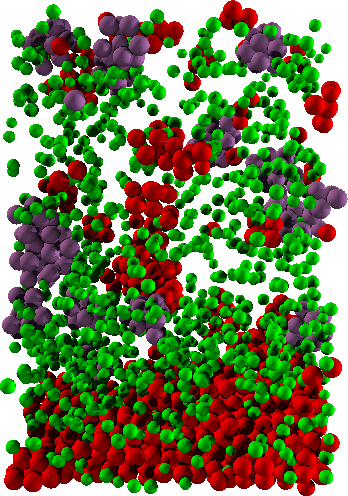
\includegraphics[height=0.6\textheight]{mrco_ico_small_t299.png}};
	\end{tikzpicture}
	
\end{frame}

\begin{frame}{Small particles must be expelled}
	\tikzsetnextfilename{crystal_growth}
	\begin{tikzpicture}
		\matrix[matrix of nodes, inner sep=1pt, ampersand replacement=\&] (a)%
		{%
			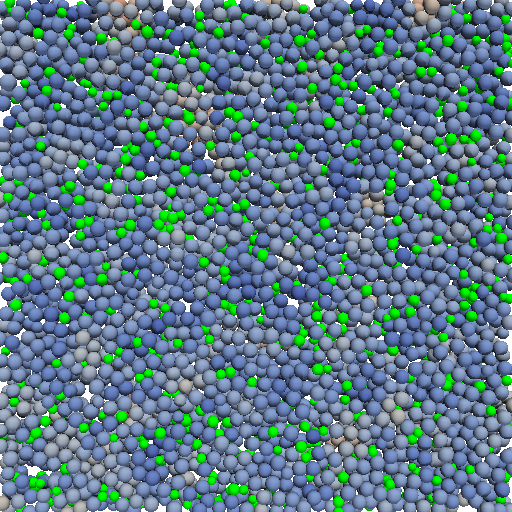
\includegraphics[width=0.25\columnwidth]{small_boo000.png} \& %
			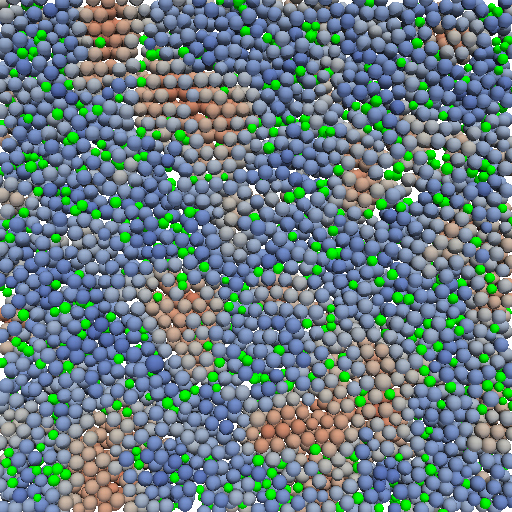
\includegraphics[width=0.25\columnwidth]{small_boo060.png} \& %
			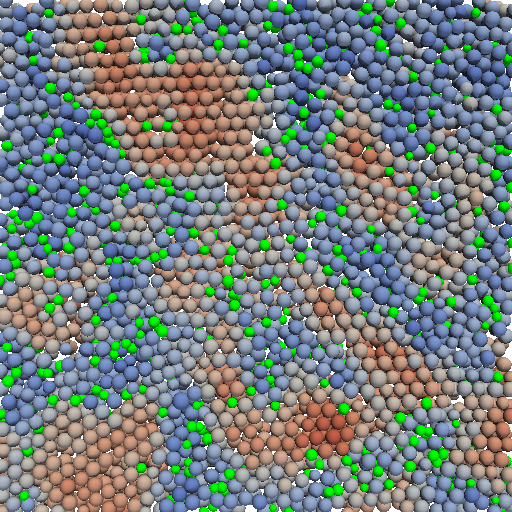
\includegraphics[width=0.25\columnwidth]{small_boo120.png}\\
			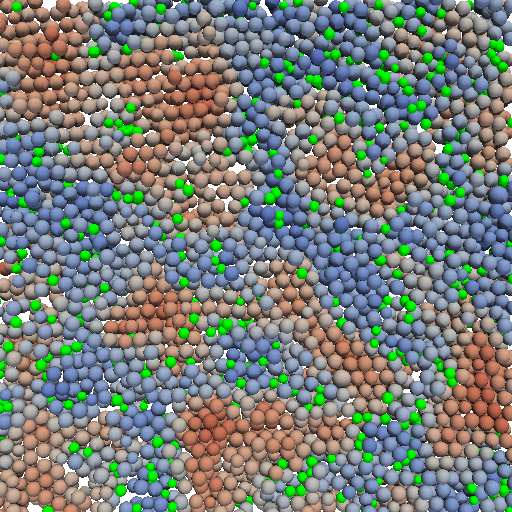
\includegraphics[width=0.25\columnwidth]{small_boo180.png} \& %
			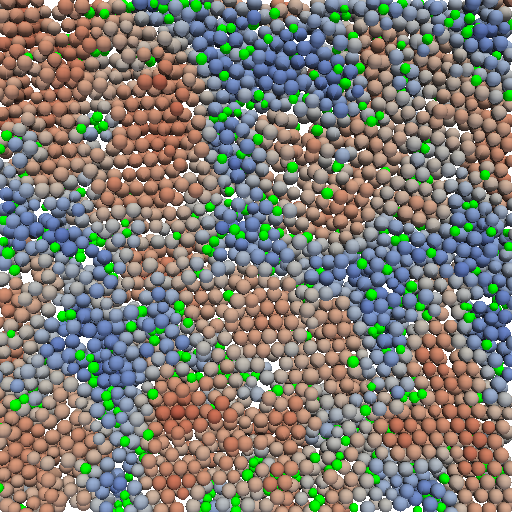
\includegraphics[width=0.25\columnwidth]{small_boo240.png} \& %
			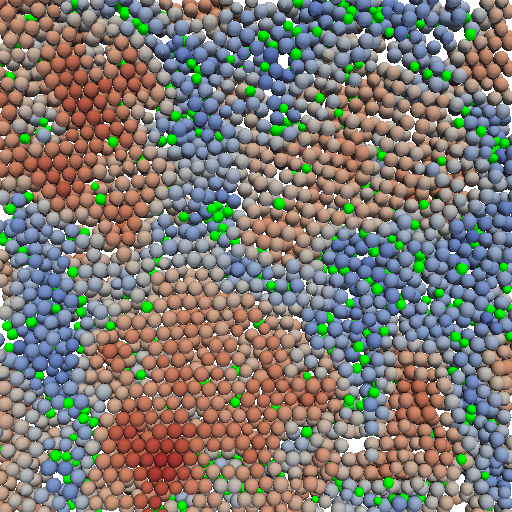
\includegraphics[width=0.25\columnwidth]{small_boo299.png}\\%
		};
		\begin{axis}[%
		name=b,
		at={(a.south east)},%
		anchor=below south west,%
		xmin=0,xmax=10, ymin=0, ymax=0.55,%
		width=5em,%
		height=0.55\columnwidth,%
		axis x line=none,%
		axis y line*=right,%
		axis on top,
		]
		\addplot graphics[xmin=0,xmax=10, ymin=0, ymax=0.55] {color_bar.png};
		\end{axis}
		\node[above= 0 of b.outer north] {$Q_6$};
	\end{tikzpicture}
	
	Every \SI{12}{\hour}
\end{frame}


\setcounter{framenumber}{\value{finalframe}}

\end{document}